\documentclass[12pt]{article}

\usepackage{amsfonts,amssymb}
\usepackage[utf8]{inputenc}
\usepackage[russian]{babel}
\usepackage{graphicx}
\usepackage{amsmath}
\usepackage{amsfonts}
\usepackage[ruled, lined]{algorithm2e}

\textheight=220mm
\textwidth=160mm

\newcommand{\sgn}{\operatorname{sgn}}
\newcommand{\argmax}{\operatorname{argmax}}
\newcommand{\NA}{\operatorname{NA}}
\newcommand{\OR}{\operatorname{ or }}
\newcommand{\LCS}{\operatorname{LCS}}
%\DeclareMathOperator{\sgn}{sgn}

\title{\bf Домашнее задание по курсу \\ <<Методы
и структуры данных поиска.>>}
\author{А.Е. Оразаев}
\date{}
\begin{document}

\voffset=-20mm
\hoffset=-12mm
\font\Got=eufm10 scaled\magstep2 \font\Got=eufm10

\maketitle

\section{Задача 3-4.}
\subsection{Описание алгоритма.}

Для решения задачи несколько модифицируем алгорит Укконена для построения
суффиксных деревьев.

Для каждой вершины $ v $ суффиксного дерева будем говорить, что $ L_{v} $ --
длина префикса определяемого текущей вершиной для своего суффикса. Простыми
словами: глубина графа выраженная в символах, а не в вершинах.

Введем следующую модификацию в алгоритм: каждый раз, добавляя новую
листовую вершину в дерево будем заполнять соответствующее поле массива
$ l $, с результатами работы алгоритма. Делать это будем вот так.

Перед началом алгоритма построения суффиксного дерева заполним весь массив
$ l $ нулями.

Пусть на шаге $ i + 1 $ нам встретился символ $ T[i + 1] = x $ и на
этом шаге нам стоит добавить листовую вершину в дерево. Заметим,
что у нас уже есть построенное суффиксное дерево $ ST_i $, которое выглядит
следующим образом.
\begin{center}
    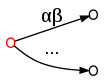
\includegraphics[width=60bp]{before_addition.png}
\end{center}

После добавления листовой вершины к вершине $ v $ дерево изменится следующим образом:
\begin{center}
    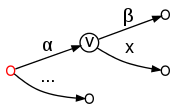
\includegraphics[width=100bp]{after_addition.png}
\end{center}

Здесь $ \alpha $ может быть не просто дугой, а путем из нескольких дуг до
вершины $ v $.  Заметим, что $ \alpha $ может быть также пустым путем, тогда
$ v $ -- это корень, $ \beta $ -- тоже пустой путь, а листовая вершина
добавляется к корню.

Далее мы пологаем $ l_{i - |\alpha| + 1} = |\alpha| $, где $ |\alpha| = L_v $.
То есть отмечаем, что в позиции $ j = i - |\alpha| + 1 $,  $ \alpha $ --
наибольшая по длинне подстрока входного текста $ T $, начинающаяся в
позиции $ j $, которая также ранее встречается в $ T $.

Утверждается, что алгоритм Укконена с введенной модификацией вычисляет
искомый массив $ l $, для текста $ T $. С поправкой на то, что в конец
текста надо добавить сэнтинел $\$$.


\subsection{Доказательство.}
\paragraph{Утверждение 1.} При добавлении листовой вершины к вершине $ v $ на шаге $ i + 1 $
описанного выше модифицированного алгоритма Укконена, $ L_v $ является
наибольшей длинной подстроки входного текста $ T $, короторая начинается в
позиции $ j = i - L_v + 1 $, а также ранее встречается в $ T $.

Допустим $ \alpha = T[j:i] $.
Пусть существует $ l_j^1 > L_v $, для которого существует $ j^1 < j $
$ T[j^1:j^1 + l_j^1 - 1] = T[j:j + l_j^1 - 1] $. Иными словами $ l_j $
мы должны положить равным $ l_j^1 $, а не $ L_v $. В таком случае
должна существовать строка $ \beta = T[j:j + l_j^1 - 1]$, которая уже
находится в суффиксном дереве полученном на шаге $ i $, так как она
встречалась ранее в тексте $ T $.
Но на шаге $ i + 1 $ мы добавляем новую вершину в дерево, а
значит, строки $ \beta $ на шаге $ i $ в дереве не было. Противоречие.


Фактически утверждение 1 гарантирует, что при добавлении листовой
вершины мы правильно заполняем соответствующее $ l_j $.


\paragraph{Утверждение 2.} После добавления вершины к корню дерева на шаге
$ i + 1 $. искомый массив $ l $ правильно заполнен для элементов с
$ 1 $ по $ i $.

Так как изначально массив $ l $ инициализирован нулями и по
утверждению 1 во всех точках, где были добавлены листовые
вершины соответствующие ячейки $ l $ заполнены верно, то нам
остается доказать, что для всех $ l_j $, где $ 1 \le j \le i $,
мы не <<забыли>> заполнить ячейки массива $ l $, то есть для
всех $ l_j $ которые должны быть больше $ 0 $, мы добавили
вершину на шаге $ j + l_j \le i + 1 $.

Очевидно, что если $ j + l_j \le i + 1 $ для конкретного $ l_j $,
то мы добавим листовую вершину на $ j + l_j $-ом шаге, так как
$ T[j:j + l_j] $ еще не присутствует в суффиксном дереве для
$ T[1:j + l_j - 1] $.

Рассмотрим случай $ j + l_j > i + 1 $
Пусть существует $ l_j $ для которого $ j + l_j > i + 1 $. В
таком случае существует $ \alpha = T[j:j + l_j - 1] $, которое
встречается в тексте $ T $ ранее позиции $ j $, отсюда следует
что $ T[i + 1] \in \alpha $ также встречается в тексте раньше
позиции $ i + 1 $, а значит по ходу алгоритма на шаге $ i + 1 $
мы не должны добавлять вершину к корню на элементе $ T[i + 1] $.
Противоречие.

Можно также легко показать, что для утверждения 2 массив $ l $
правильно заполнен с $ 1 $ по $ i + 1 $, но это нам не нужно,
так как в конце входного текста мы добавляем сэнтинел получая
текст длины $ |T| + 1 $, подавая на вход алгоритму этот текст
мы по утверждению 2 получим правильно заполненный искомый массив
$ l $ от $ 1 $ до $ |T| $, так как сэнтинел обязательно добавит
вершину к корню, как не встречавшийся ранее символ.

\subsection{Сложность}
Сложность по времений $ O(N) $.
Сложность по памяти $ O(N) $.

\end{document}
